 \documentclass[12pt]{article}
\usepackage{fontspec}
\usepackage{graphicx}
\usepackage{geometry}
\usepackage{float}
\usepackage{hyperref}
\usepackage{tikz}
\usepackage{polyglossia}
\setmainlanguage{farsi}
\setotherlanguage{english}
\newfontfamily\englishfont{Times New Roman}
\newfontfamily\persianfont[Script=Arabic]{XB Zar.ttf}




\geometry{a4paper, margin=2.5cm}
\usepackage{setspace}
\onehalfspacing
\usepackage{titling}
\usepackage{etoolbox}
\usepackage[backend=biber,style=numeric,sorting=none]{biblatex}
%%%%%%%%%%%%%%%%%%%%%%%%%%%%%%%%%%%%%%%%%%%%%%%%%%%%%%%%%%%%%%%%%%%%%%%%%%%%%
\makeatletter
\newcommand{\persiandigit}[1]{%
	\ifcase#1 ۰\or ۱\or ۲\or ۳\or ۴\or ۵\or ۶\or ۷\or ۸\or ۹\fi
}
\DeclareFieldFormat{labelnumber}{\persiandigit{#1}}
\makeatother
%%%%%%%%%%%%%%%%%%%%%%%%%%%%%%%%%
\newcommand{\persianordinal}[1]{%
	\ifcase#1
	\or اول%
	\or دوم%
	\or سوم%
	\or چهارم%
	\or پنجم%
	\or ششم%
	\or هفتم%
	\or هشتم%
	\or نهم%
	\or دهم%
	\or یازدهم%
	\or دوازدهم%
	\or سیزدهم%
	\or چهاردهم%
	\or پانزدهم%
	\or شانزدهم%
	\or هفدهم%
	\or هجدهم%
	\or نوزدهم%
	\or بیستم%
	\else #1\fi
}

\newcommand{\persianordinalpage}{\persianfont\persianordinal{\value{page}}}


%%%%%%%%%%%%%%%%%%%%%%%%%%%%%%%%%%%%%%%%%%%%%%%%%%%%%%%%%%%%%%%%%%%%%%%%%%%%%
\begin{filecontents}{\jobname.bib}
@online{opengroup-dlsym,
    author    = {{The Open Group}},
    title     = {dlsym — Dynamic Linker Function},
    year      = {2024},
    url       = {https://pubs.opengroup.org/onlinepubs/009604299/functions/dlsym.html},
    note      = {Accessed: 2025-08-17}
}

@online{opengroup-readdir,
    author    = {{The Open Group}},
    title     = {readdir — Directory Reading Function},
    year      = {2024},
    url       = {https://pubs.opengroup.org/onlinepubs/7908799/xsh/readdir.html},
    note      = {Accessed: 2025-08-17}
}

@online{geeksforgeeks-shared-libraries,
    author    = {{GeeksforGeeks contributors}},
    title     = {Working with Shared Libraries — Set 2},
    year      = {2025},
    url       = {https://www.geeksforgeeks.org/operating-systems/working-with-shared-libraries-set-2/},
    note      = {Accessed: 2025-08-17}
}

@online{gnu-coreutils-ls,
    author    = {{GNU Coreutils contributors}},
    title     = {ls.c — Source code of ls command},
    year      = {2025},
    url       = {https://cgit.git.savannah.gnu.org/cgit/coreutils.git/tree/src/ls.c},
    note      = {Accessed: 2025-08-17}
}

@online{sourcerer-kernel-module,
    author    = {Robert W. Oliver II},
    title     = {Writing a Simple Linux Kernel Module},
    year      = {2017},
    url       = {https://blog.sourcerer.io/writing-a-simple-linux-kernel-module-d9dc3762c234},
    note      = {Accessed: 2025-08-17}
}

@online{github-issue-kallsyms,
    author    = {xcellerator},
    title     = {kallsyms\_lookup\_name is not exported anymore in kernels > 5.7},
    year      = {2021},
    url       = {https://github.com/xcellerator/linux_kernel_hacking/issues/3},
    note      = {Accessed: 2025-08-17}
}

\end{filecontents}

\addbibresource{\jobname.bib}

\defbibheading{bibliography}[]{%
	\begin{RTL}
		\section*{مراجع}
	\end{RTL}
}

%%%%%%%%%%%%%%%%%%%%%%%%%%%%%%%%%%%%%%%%%%%%%%%%%%%%%%%%%%%%%%%%%%%%%%%%%%%%%

\begin{document}
	
	% ==============================
	% Title Page
	% ==============================
	\begin{titlepage}
		\centering
		\vspace*{1cm}
		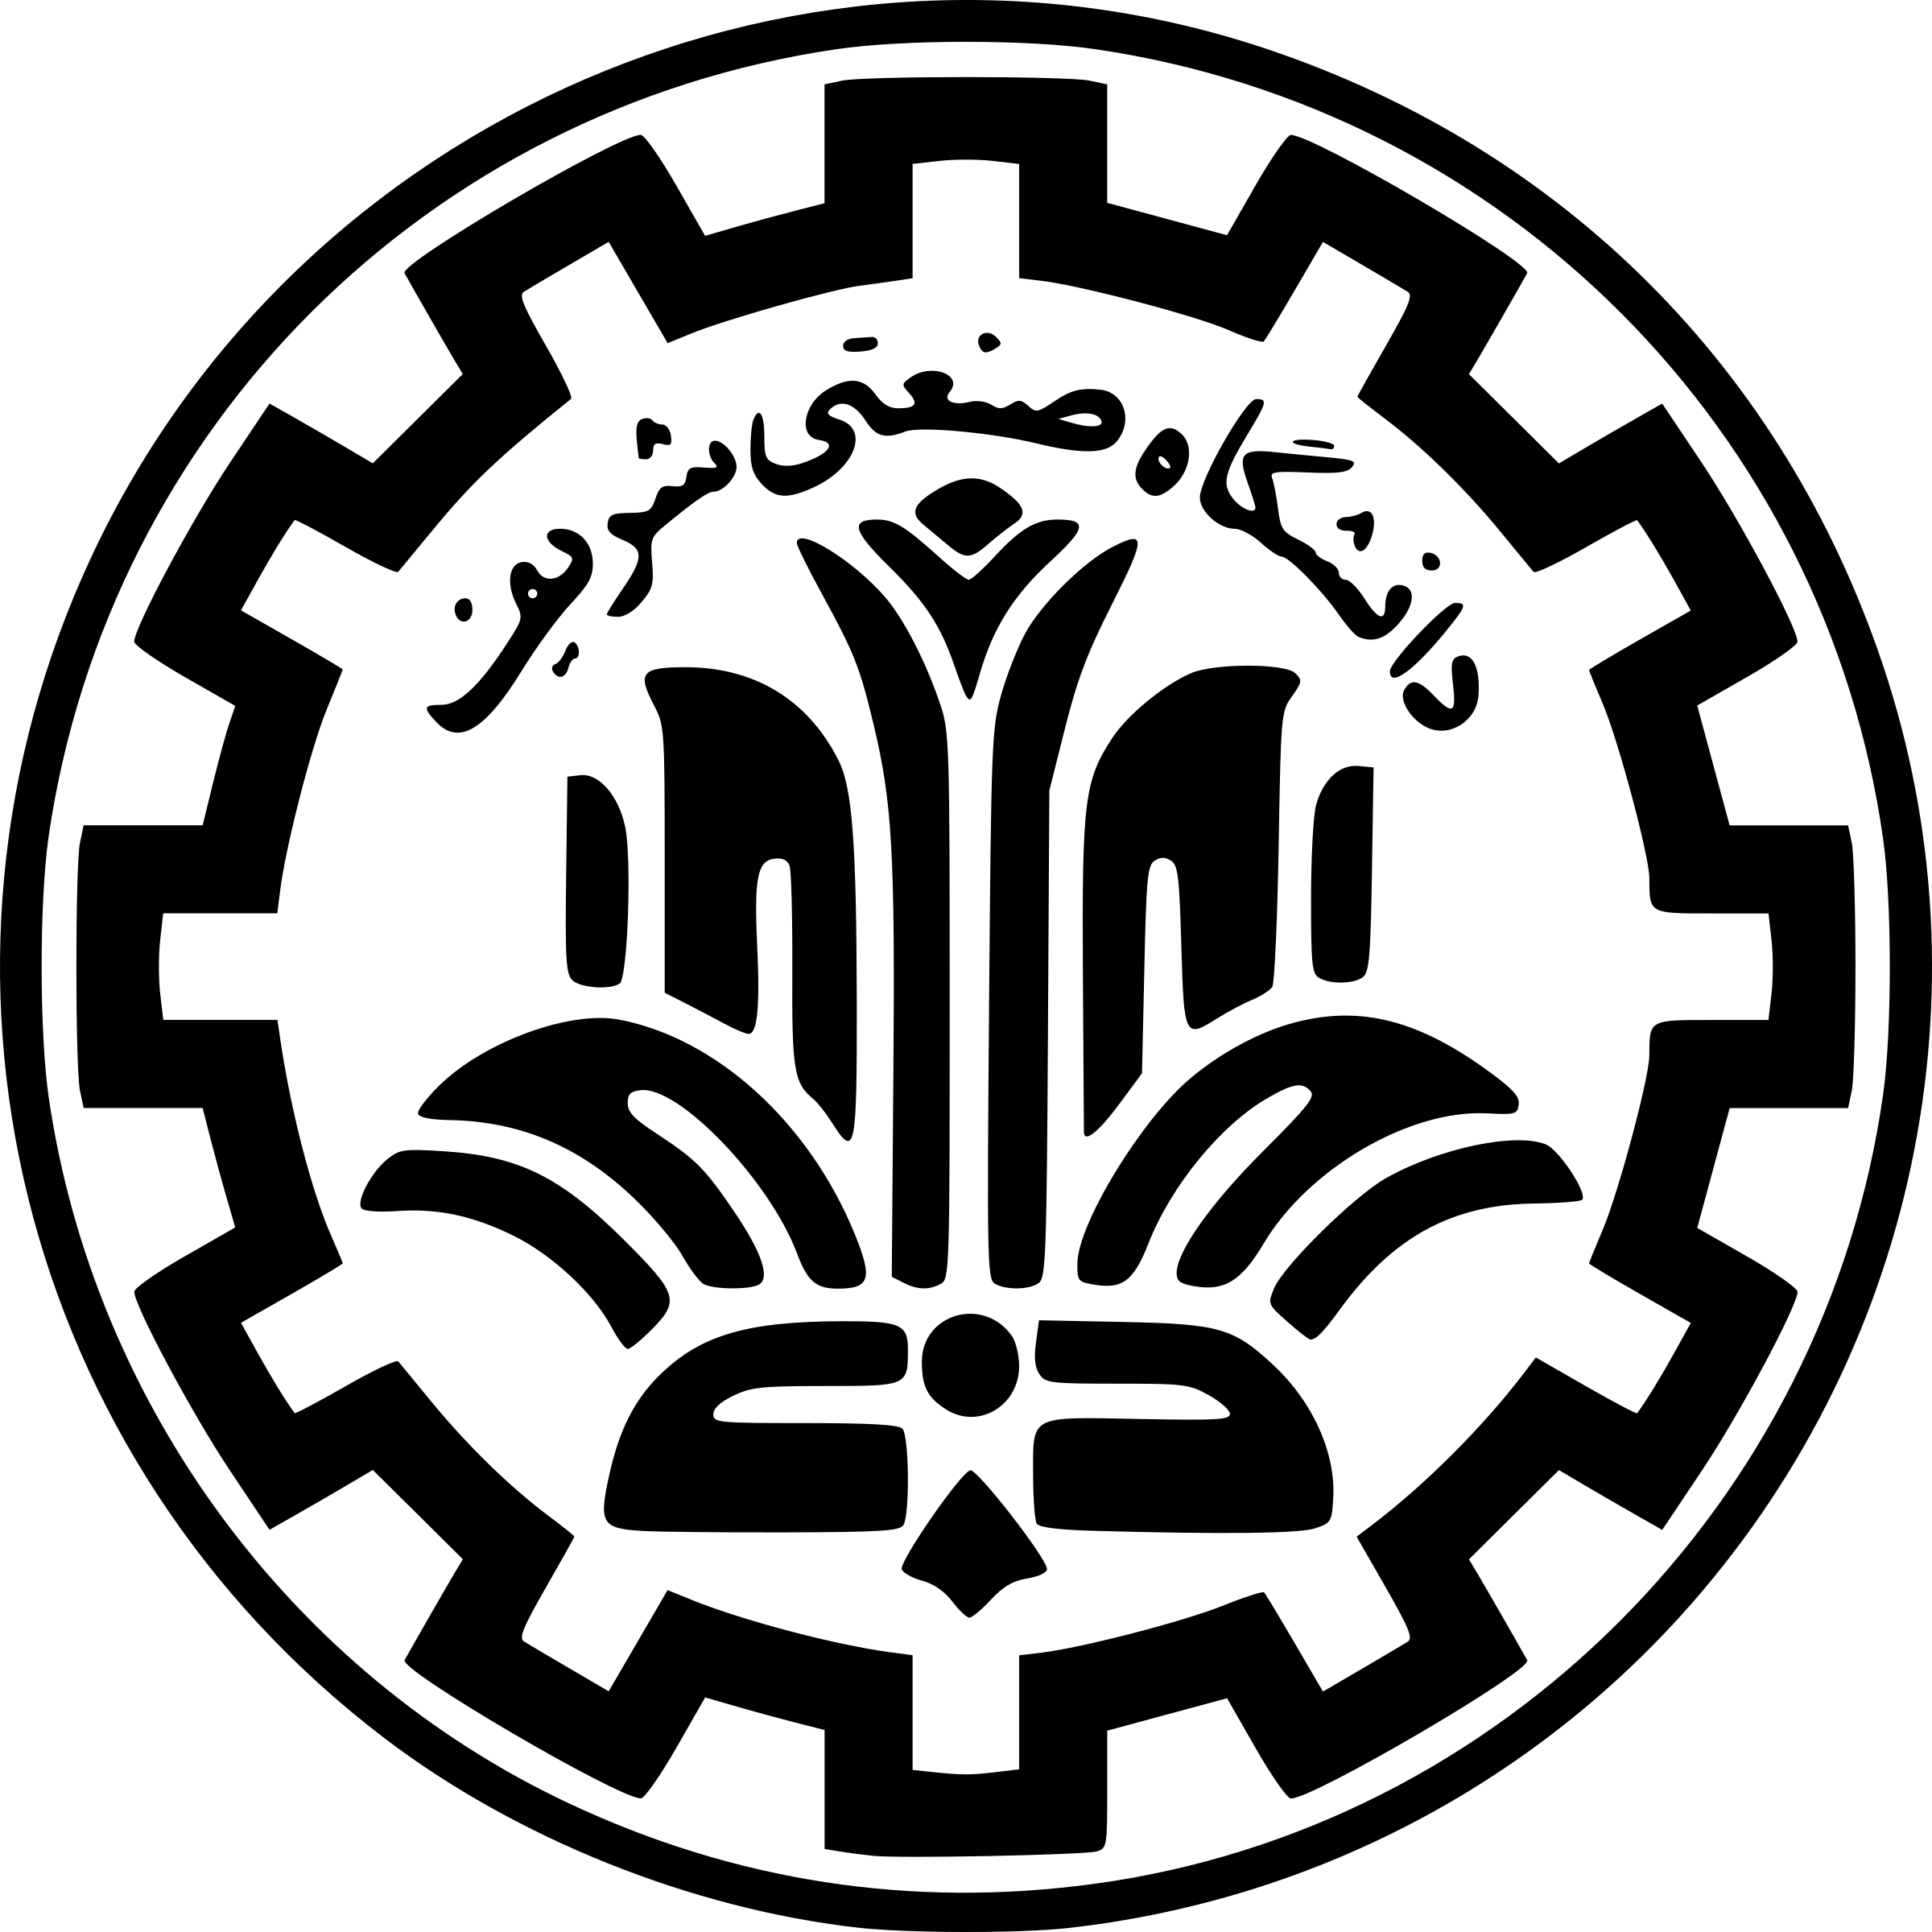
\includegraphics[width=4cm]{sharif.png}\\[1.5cm]
		{\Large\textbf{دانشگاه صنعتی شریف}}\\[0.5cm]
		{\large\textbf{دانشکده‌ی مهندسی کامپیوتر}}\\[1.5cm]
		{\Huge\textbf{گزارش کار آزمایشگاه}}\\[0.5cm]
		{\LARGE\textbf{آزمایشگاه سیستم‌های عامل}}\\[2cm]
		
		\textbf{گزارش آزمایش شماره ۸}\\
		(آشنایی با توابع سیستمی)
		
		\vfill
		\begin{tabular}{rl}
			\textbf{شماره‌ی گروه:} & ۲۰ \\
			\textbf{گروه:} &
			ارشیا یوسف‌نیا (۴۰۱۱۱۰۴۱۵) \\
			& محمدعارف زارع زاده (۴۰۱۱۰۶۰۱۷) \\
			\textbf{استاد درس:} & دکتر بیگی \\
			\textbf{تاریخ:} & تابستان ۱۴۰۴ \\
		\end{tabular}
	\end{titlepage}
	
	% ==============================
	% Persian Ordinal Page Numbering
	% ==============================
	\clearpage
	\setcounter{page}{1}
	\renewcommand{\thepage}{\persianordinalpage}
	
	\tableofcontents
	\clearpage
	\listoffigures
	% \clearpage
	% \listoftables
	
	% ==============================
	% Switch to Persian Digits (۱, ۲, ۳, ...)
	% ==============================
	\clearpage
	\setcounter{page}{1}
	\pagenumbering{arabic}
	\renewcommand{\thepage}{\persianfont\arabic{page}}
	
	
	% ==============================
	% Main Content
	% ==============================
        \section{آزمایش ۱}

        \subsection{توضیح کد}
        در آدرس 
        \textenglish{source code/part1/sysaddr.c}
        می‌توان کد کامل ماژول هسته را مشاهده کرد.
        در ادامه، بخش‌های مهم آن را توضیح می‌دهیم.

        در
        \cite{sourcerer-kernel-module}
        که در گیتهاب درس به عنوان راهنما داده شده بود، نحوه‌ی کلی نوشتن ماژول سطح هسته و اجرای آن را توضیح می‌دهد. در نوشتن کد این بخش، از اصول و مثال‌های آن کمک می‌گیریم.

        برای مشاهده‌ی توابع سطح سیستم، می‌توان از
        \textenglish{syscall\_table}
        که با کمک تابع
        \textenglish{kallsyms\_lookup\_name}
        می‌توان آن را پیدا کرد،
        استفاده کرد. برای مشاهده‌ی آدرس و نام و سایر اطلاعات 
        آنها از تابع
        \textenglish{kallsyms\_lookup}
        می‌توان استفاده کرد. از آنجایی که در نسخه‌های جدید لینوکس آنها به طور مستقیم وجود ندارند، باید آنها را با استفاده از
        \textenglish{kprobe}
        دریافت کرد
        \cite{github-issue-kallsyms}.

        با روشی مشابه
        \cite{github-issue-kallsyms}
        تابعی می‌سازیم که با کمک
        \textenglish{kprobe}
        مواردی که می‌خواهیم را به ما دهد. آن را در شکل
        \ref{im1}
        می‌توان مشاهده کرد.

        \begin{figure}[H]
		\centering
		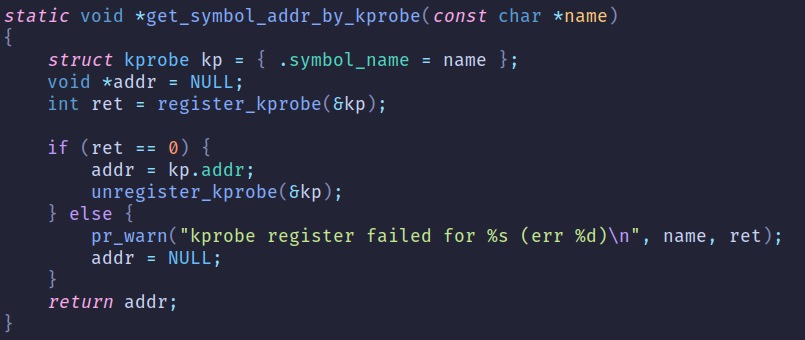
\includegraphics[width=0.8\textwidth]{report8-resources/1.png}
		\caption{تابع کمکی دریافت خواسته‌ها با کمک \textenglish{kprobe}}
            \label{im1}
	\end{figure}

        سپس در تابع 
        \textenglish{\_\_init}
        ابتدا مواردی که می‌خواهیم را با کمک این تابع کمکی دریافت کرده (نیمه‌ی اول تابع)، سپس نام و آدرس توابع سیستمی را دریافت می‌کنیم (نیمه‌ی دوم).
        نیمه‌ی اول این تابع در شکل
        \ref{im2}
        و نیمه‌ی دوم آن در شکل
        \ref{im3}
        قابل مشاهده است.
        در ادامه‌، این دو نیمه را توضیح می‌دهیم.

        \begin{figure}[H]
		\centering
		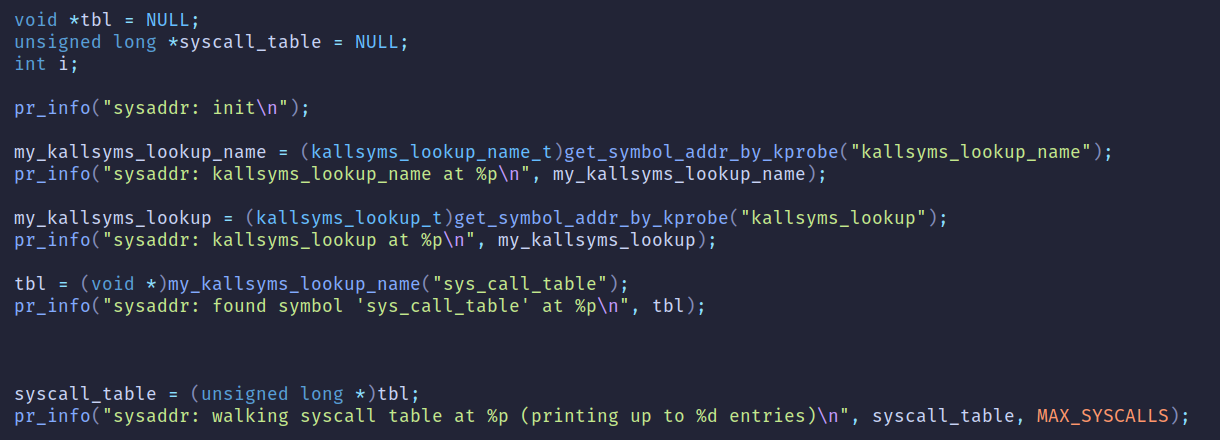
\includegraphics[width=0.8\textwidth]{report8-resources/2.png}
		\caption{نمیه‌ی اول تابع \textenglish{\_\_init} در فایل \textenglish{sysaddr.c}}
            \label{im2}
	\end{figure}

        \begin{figure}[H]
		\centering
		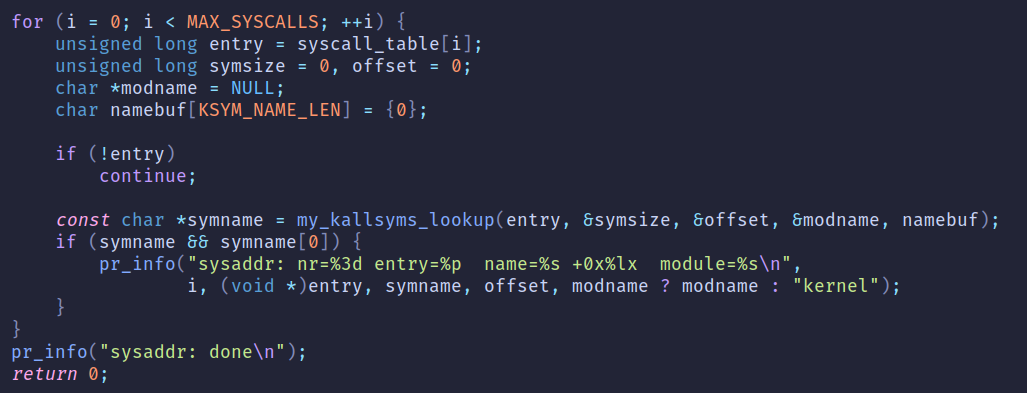
\includegraphics[width=0.8\textwidth]{report8-resources/3.png}
		\caption{نمیه‌ی دوم تابع \textenglish{\_\_init} در فایل \textenglish{sysaddr.c}}
            \label{im3}
	\end{figure}

        در شکل
        \ref{im2}
        ابتدا تابع
        \textenglish{kallsyms\_lookup\_name}
        را دریافت کرده که با کمک آن،
        \textenglish{sys\_call\_table}
        که تمام توابع سیستمی در آن قرار دارند را دریافت کنیم. سپس تابع
        \textenglish{kallsyms\_lookup}
        که با کمک آن می‌توان نام و آدرس و سایر موارد مربوط به توابع 
        سیستمی را دریافت کرد را با کمک تابع کمکی بالا دریافت می‌کنیم.

        در شکل
        \ref{im3}
        روی تمام توابع یک حلقه اجرا کرده تا نام و آدرس و سایر موارد مربوط به آنها را چاپ کنیم. در آن ابتدا متغیرهای خالی تعریف کرده، سپس به تابع
        \textenglish{kallsyms\_lookup}
        آنها را می‌دهیم تا پر کند. سپس آنها را چاپ می‌کنیم.

        درنهایت، تابع
        \textenglish{\_\_exit}
        را تعریف کرده که اتمام کار ماژول را گزارش می‌کند، و درنهایت
        \textenglish{\_\_init}
        و 
        \textenglish{\_\_exit}
        را به عنوان ماژول تعریف می‌کنیم.

        \subsection{نحوه‌ی اجرا و نیازمندی‌ها}

        برای اجرای این کد، موارد زیر با این دستور باید نصب شوند:

        \begin{english}
            sudo apt install make build-essential linux-headers-`uname -r`
        \end{english}

        همچنین برای اجرای کد، لازم است طبق
        \cite{sourcerer-kernel-module}
        یک 
        \textenglish{Makefile}
        درست کنیم. این 
        \textenglish{Makefile}
        درست مانند منبع است، فقط یک بخش تست هم به آن اضافه کردیم که تست کردن این کد راحت تر شود. در بخش تست آن، ابتدا 
        \textenglish{dmesg}
        خالی می‌شود. سپس ماژول اضافه می‌شود و یک ثانبه صبر می‌کند تا ماژول به طور کامل اجرا شود، سپس محتویات 
        \textenglish{dmesg}
        نشان داده می‌شود و در نهایت، ماژول حذف می‌شود. در شکل 
        \ref{im10}
        می‌توان محتویات
        \textenglish{Makefile}
        را دید. همچنین در آدرس
        \textenglish{source code/part1}
        نیز وجود دارد.

        \begin{figure}[H]
		\centering
		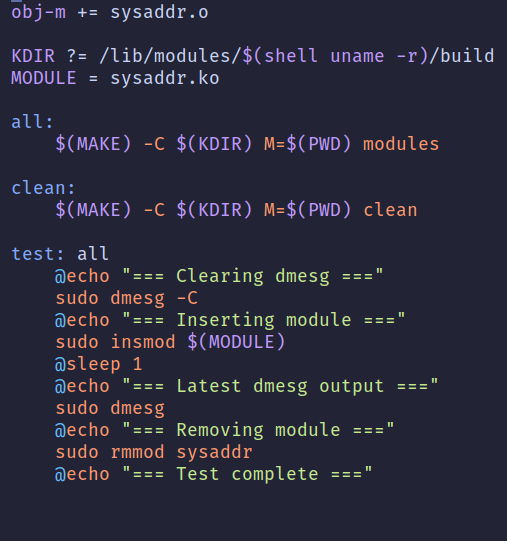
\includegraphics[width=0.8\textwidth]{report8-resources/10.png}
		\caption{محتویات \textenglish{Makefile}}
            \label{im10}
	\end{figure}

        برای اجرای آن، ابتدا باید دستور
        \textenglish{make}
        را زد، و سپس با
        \textenglish{make test}
        آن را تست کرد.

        \subsection{خروجی}
        در شکل‌های 
        \ref{im5}
        و 
        \ref{im6}
        می‌توان خروجی آن را دید. چون کل خروجی در شکل
        \ref{im6}
        قابل مشاهده نیست، خروجی کامل تست را در آدرس
        \textenglish{source code/part1/output.txt}
        می‌توان مشاهده کرد.

        \begin{figure}[H]
		\centering
		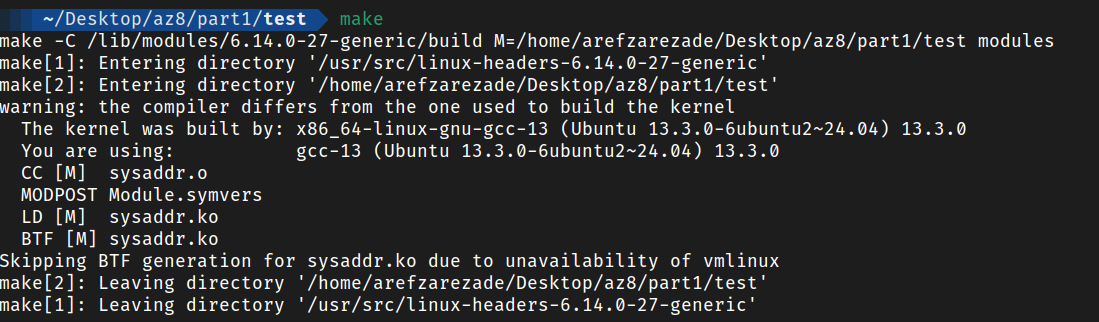
\includegraphics[width=0.8\textwidth]{report8-resources/5.png}
		\caption{کامپایل کد ماژول هسته}
            \label{im5}
	\end{figure}

        \begin{figure}[H]
		\centering
		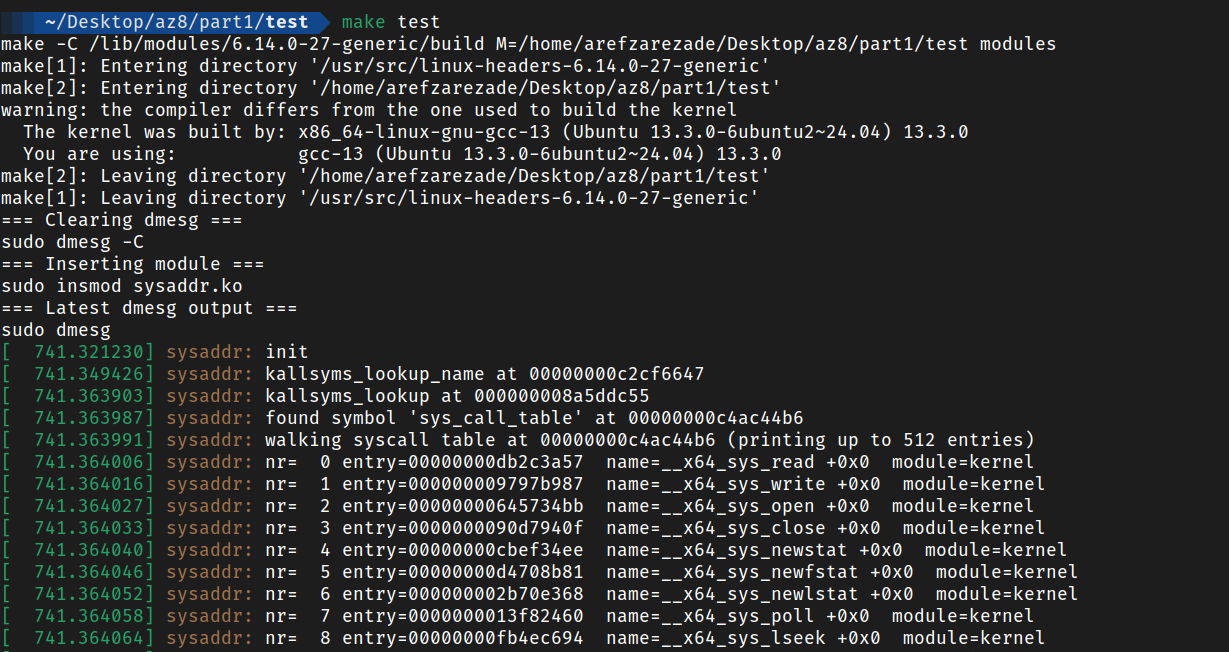
\includegraphics[width=0.8\textwidth]{report8-resources/6.png}
		\caption{اجرای کد ماژول هسته}
            \label{im6}
	\end{figure}
        
        

        \section{آزمایش ۲}

        \subsection{توضیح کد}

        برای اینکه با 
        \textenglish{LD\_PRELOADING}
        بتوانیم عملکرد دستور
        \textenglish{ls}
        را تغییر دهیم، ابتدا باید بررسی کنیم که این دستور از چه توابعی استفاده می‌کند، سپس یک کد به زبان
        \textenglish{C}
        بنویسیم که تابعی هم‌نام با تابعی که دستور
        \textenglish{ls}
        با کمک آن محتویات یک دایرکتوری را پیدا می‌کند ساخته و عملکرد آن را به صورت مورد نظر خودمان تغییر دهیم. درنهایت، آن را به فرمت مناسب برای کتابخانه‌های مشترک در آورده و کاری کنیم که دستور 
        \textenglish{ls}
        آن را به عنوان کتابخانه‌ی مشترک، قبل از بقیه‌ی کتابخانه‌های مشترک لود کند. اینگونه، 
        \textenglish{linker}
        تابع ساخته شده‌ی ما را به جای تابع اصلی به دستور 
        \textenglish{ls}
        می‌دهد.
        

        طبق
        \cite{gnu-coreutils-ls}
        می‌دانیم که دستور
        \textenglish{ls}
        از تابع
        \textenglish{readdir}
        برای خواندن محتوای یک دایرکتوری استفاده می‌کند.
        در شکل‌های 
        \ref{im8}
        و 
        \ref{im9}
        می‌توانیم تابع 
        \textenglish{readdir}
        جدید که ساخته‌ایم را مشاهده کنیم. همچنین در آدرس
        
        \begin{english}
            source code/part2/fake\_ls.c
        \end{english}

        \noindent
        فایل کامل این کد قرار دارد. در ادامه‌ی گزارش، بخش‌های اصلی این کد را توضیح می‌دهیم.

        \begin{figure}[H]
		\centering
		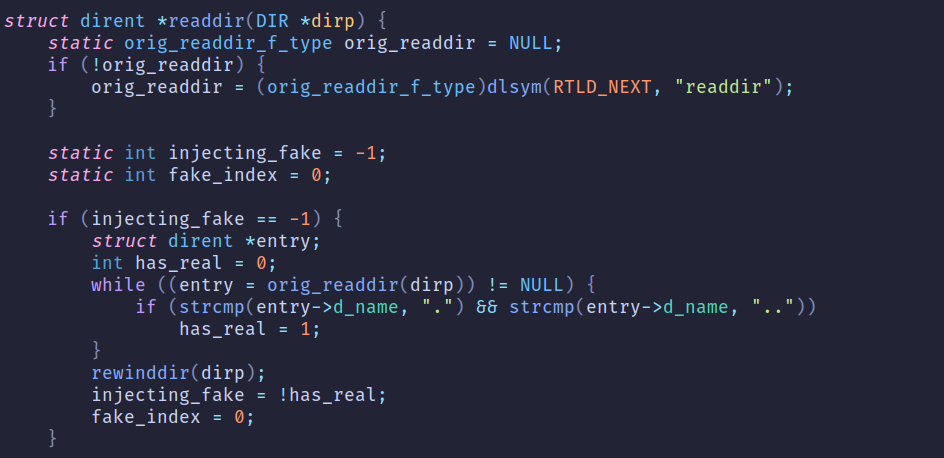
\includegraphics[width=0.8\textwidth]{report8-resources/8.png}
		\caption{نیمه‌ی اول تابع \textenglish{readdir} جدید}
            \label{im8}
	\end{figure}

        \begin{figure}[H]
		\centering
		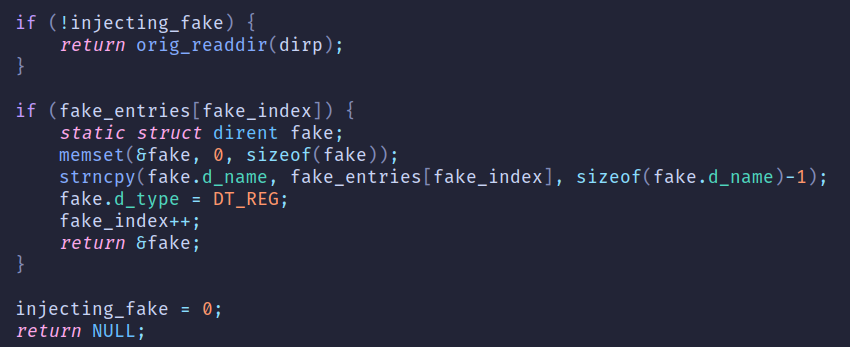
\includegraphics[width=0.8\textwidth]{report8-resources/9.png}
		\caption{نیمه‌ی دوم تابع \textenglish{readdir} جدید}
            \label{im9}
	\end{figure}

        می‌دانیم تابع
        \textenglish{readdir}
        اصلی، با هربار اجرا شدن، یکی دیگر از فایل‌های موجود در دایرکتوری را خروجی می‌دهد، تا وقتی که فایل دیگری نباشد، که در آن زمان
        \textenglish{NULL}
        را خروجی می‌دهد
        \cite{opengroup-readdir}.
        پس تابع ما نیز طبق خواسته‌ی صورت آزمایش در کوئرا، ابتدا بررسی می‌کند که دایرکتوری خواسته شده خالی است یا نه. برای این کار، ابتدا تابع 
        \textenglish{readdir}
        اصلی را با کمک تابع
        \textenglish{dlsym}
        از کتابخانه‌ی
        \textenglish{libdl}
        را پیدا می‌کنیم. آرگومان
        \textenglish{RTLD\_NEXT}
        باعث می‌شود که دفعه‌ی بعدی که این تابع در کتابخانه‌های مشترک دیده شود خروجی داده شود
        \cite{opengroup-dlsym}.
        سپس، متغیر 
        \textenglish{static}
        به نام
        \textenglish{injecting\_fake}
        با مقدار اولیه‌ی 
        \textenglish{-1}
        ساخته و اگر مقدار آن هنوز 
        \textenglish{-1}
        باشد، به آن مقدار مناسب می‌دهیم. دلیل پیاده سازی به این صورت این است که 
        دستور
        \textenglish{ls}
        این تابع را یک بار لود کرده و چند بار اجرا می‌کند. 
        پس مقدار مناسب به این متغیر، فقط در دفعه‌ی اول اجرا داده می‌شود. 

        برای بررسی اینکه دایرکتوری خالی است یا خیر، با تابع
        \textenglish{readdir}
        بررسی می‌کنیم که خروجی‌ای به جز
        \textenglish{.}
        و
        \textenglish{..}
        در آن دایرکتوری است یا نه.
        اگر باشد، یعنی دایرکتوری خالی نیست.

        سپس طبق شکل
        \ref{im9}
        اگر دایرکتوری خالی نباشد، خروجی‌ تابع
        \textenglish{readdir}
        اصلی را می‌دهیم. در غیر این صورت، تعدادی فایل جعلی (که در یک آرایه از رشته ذخیره کرده‌ایم) را خروجی می‌دهد. این دقیقا مطابق خواسته‌ی کوئرا است که در صورت خالی بودن دایرکتوری، محتوای جعلی نشان داده شوند و در صورت خالی نبودن محتوای اصلی.

        در نهایت نیز
        \textenglish{NULL}
        را خروجی می‌دهیم که به دستور
        \textenglish{ls}
        نشان دهیم تمام فایل‌های دایرکتوری نشان داده شده اند.

        \subsection{نحوه‌ی اجرا و دیدن عملکرد کد}
        برای اینکه این کد را به فرمت مناسب برای کتابخانه‌های مشترک کامپایل کنیم، به 
        \textenglish{gcc}
        باید دو فلگ
        \textenglish{-shared}
        و 
        \textenglish{-fPIC}
        را اضافه کنیم
        \cite{geeksforgeeks-shared-libraries}.
        اولی به 
        \textenglish{gcc}
        می‌گوید که آن را به صورت کتابخانه‌ی مشترک کامپایل کند، نه فایل اجرایی. دومی هم به
        \textenglish{gcc}
        می‌گوید که آن را به صورت
        \textenglish{position independent}
        کامپایل کند، به این صورت که آدرس‌های مورد استفاده در کد، وابسته به موقعیت برنامه در حافظه هنگام اجرا نباشد. این به این دلیل مهم است که کتابخانه‌های مشترک در هر زمان و در هرجایی از حافظه ممکن است لود شوند.

        همچنین چون از کتابخانه‌ی 
        \textenglish{libdl}
        استفاده شده است، باید تگ
        \textenglish{-ldl}
        را هنگام کامپایل اضافه کنیم. یک نمونه‌ی مناسب کامپایل این کد به صورت زیر است:

        \begin{english}
            gcc -Wall -fPIC -shared -o fake\_ls.so fake\_ls.c -ldl
        \end{english}
        
        سپس باید کاری کنیم که این کتابخانه‌ی مشترک لود شود. راحت ترین راه برای این کار این است که آدرس خروجی کامپایل را در فایل 
        \textenglish{/etc/ld.so.preload}
        اضافه کنیم. آن را در شکل
        \ref{im7}
        می‌توانید مشاهده کنید.

        \subsection{خروجی کد}
        در شکل 
        \ref{im7}
        می‌توانید عملکرد درست این کد را مشاهده کنید. ابتدا دستور 
        \textenglish{ls}
        روی همان دایرکتوری اجرا می‌شود. از آنجایی که آن دایرکتوری خالی نیست، محتوای واقعی آن نمایش داده می‌شود. سپس یک دایرکتوری خالی ساخته می‌شود و دستور 
        \textenglish{ls}
        روی آن اجرا می‌شود. همانطور که می‌توان مشاهده کرد، محتوای جعلی نمایش داده می‌شوند.

        \begin{figure}[H]
		\centering
		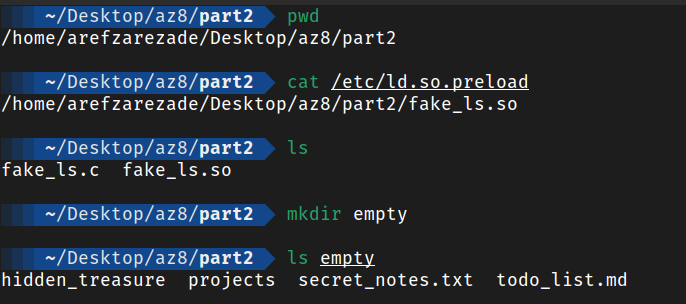
\includegraphics[width=0.8\textwidth]{report8-resources/7.png}
		\caption{بررسی درستی عملکرد خواسته‌ی آزمایش دوم}
            \label{im7}
	\end{figure}
	
	% ==============================
	% References
	% ==============================
	\newpage
	\begin{LTR}
		\begin{english}
\printbibliography[title={مراجع}]
\end{english}
	\end{LTR}

	
\end{document}

